Il transistore MOSFET (\emph{Metal-Oxide Semiconductor Field-Effect Transistor}) è un dispositivo elettronico utilizzato sia in circuiti digitali, principalmente come interruttore controllato in tensione, sia in circuiti analogici, come amplificatori di segnale o come resistenze controllate in tensione.\\

\begin{figure}[H]
  \centering
  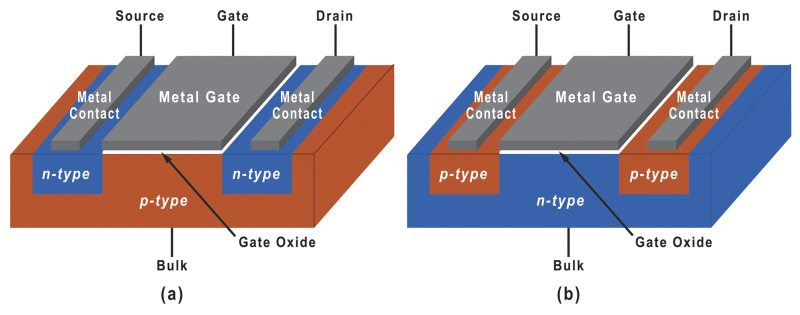
\includegraphics[width=0.80\textwidth]{./capitolo1/MOSFET/StrutturaMosfet}
  \caption[Struttura dei MOSFET]{MOSFET a canale N (a) e a canale P (b)}
  \label{fig:StrutturaMosfet}
\end{figure}

Come mostrato nella figura \ref{fig:StrutturaMosfet}, i MOSFET sono caratterizzati da quattro terminali: Source (S), Drain (D), Gate (G) e Bulk (B).
Il MOSFET a canale N viene realizzato su un substrato di tipo P in cui sono innestate due regioni fortemente drogate di tipo N. Queste due regioni presentano delle metallizzazioni che formano i terminali di Source e di Drain. Sul substrato, tra le due regioni fortemente drogate, è presente un sottile strato di ossido che fa da isolante (storicamente $SiO_2$, attualmente si usano anche altri ossidi) sopra il quale si trova una metallizzazione che forma il contatto di Gate. Il Bulk (o Substrato) è il terminale che si collega solitamente con il Source.\\

\subsection{Regioni di funzionamento e caratteristica $I-V$}

\begin{figure}[H]
  \centering
  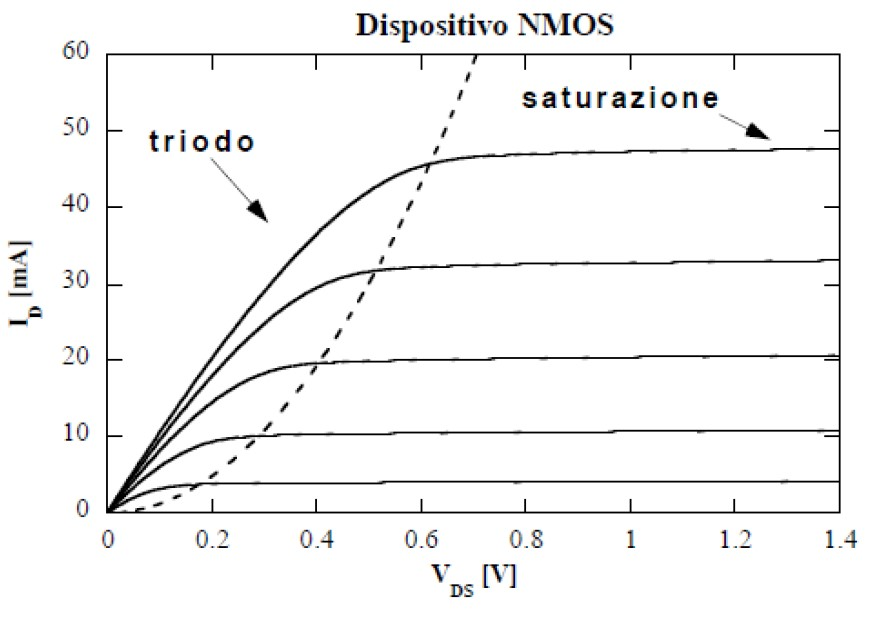
\includegraphics[width=0.80\textwidth]{./capitolo1/MOSFET/Caratteristica-I-V}
  \caption[Caratteristica $I-V$ di un MOSFET a canale N]{Caratteristica $I-V$ di un MOSFET a canale N}
  \label{fig:caratteristica-I-V}
\end{figure}

In un MOSFET a canale N, in linea generale, può scorrere una corrente $I_D$ che va dal Drain al Source in funzione di due tensioni (sempre non negative): 
\begin{itemize}
  \item la tensione presente tra Drain e Source ($V_{DS}$);
  \item la tensione presente tra Gate e Source ($V_{GS}$).  
\end{itemize}

La dipendenza di $I_D$ da tali tensioni è messa in evidenza dalla caratteristica corrente-tensione (figura \ref{fig:caratteristica-I-V}).

Quando $V_{GS} = 0$, indipendentemente dal valore di $V_{DS}$, la corrente $I_D$ è nulla, poiché la giunzione P-N composta da substrato e Drain e quella formata da substrato e Sourse sono in regione inversa. \\
Aumentando il valore di $V_{GS}$, le lacune presenti nel substrato si allontanano dalla regione direttamente al di sotto dell'ossido, creando una
zona svuotata di portatori di carica liberi. Gli elettroni presenti nel semiconduttore
vengono attirati creando una regione di canale di tipo N che unisce il
Source e il Drain. Questo canale permette il passaggio di corrente, ma per crearlo è necessario che $V_{GS}$ abbia un valore almeno pari alla cosiddetta tensione di soglia ($V_{th}$). Finché $V_{GS} < V_{th}$, il MOSFET si trova in regione di \emph{cutoff} e $I_D \simeq 0$.

Nel momento in cui $V_{GS}$ eguaglia e supera $V_{th}$, il canale di conduzione è completo e inizia a scorrere corrente, seguendo leggi matematiche differenti in funzione del valore di $V_{DS}$.\\

Se $V_{DS} < V_{GS} -  V_{th}$, il MOSFET è in regione lineare o di triodo e la corrente di Drain segue la seguente legge:\\
\centerline{ $I_D = 2k_n\left[ \left(V_{GS}-V_{th}\right)V_{DS} - \frac{V_{DS}^2}{2}\right]$}

dove

\begin{align*}
   k_n &= \frac{1}{2}\mu_n C_{ox}\frac{W}{L} \\
   \mu_n &= \text{mobilità degli elettroni} \\
   C_{ox} &= \text{capacità dell'ossido} \\
   W &= \text{larghezza del canale} \\
   L &= \text{lunghezza del canale}
\end{align*}

Se, invece, $V_{DS} > V_{GS} -  V_{th}$ il MOSFET si trova in regione di saturazione e la corrente di Drain ha un andamento lineare che segue la legge:\\
\centerline{ $I_D = k_n\left(V_{GS}-V_{th}\right)^2 (1+\lambda V_{DS})$}\\
dove $\lambda$ è un fattore matematico ricavato dalla caratteristica I-V ottenuta sperimentalmente.\\

Tutto quanto detto finora sui MOSFET a canale N vale in maniera analoga per i MOSFET a canale P.
Altri parametri verranno descritti nel prossimo capitolo.

\subsection{Modello per piccolo segnale e sorgenti di rumore}
Il modello per piccolo segnale rappresenta il funzionamento del MOSFET nel momento in cui si fissa il punto di lavoro in continua e si fornisce in ingresso al dispositivo un segnale con un'ampiezza sufficientemente piccola da non alterarne il funzionamento. \\

In prima approssimazione, il MOSFET si comporta come un generatore di corrente controllato in tensione che emette una corrente proporzionale al valore di $V_{GS}$. La costante di proporzionalità è la transconduttanza di canale $g_m$, che dipende dal punto di lavoro ed è descritta meglio al paragrafo \ref{sec:transconduttanza}. Un modello più accurato prevede che, quando il MOSFET è in saturazione, la corrente di Drain dipenda anche da $V_{DS}$ in modo lineare. Nel circuito equivalete per piccolo segnale, perciò, in parallelo al generatore di corrente, è presente una resistenza $r_0 = \frac{1}{\lambda I_{D,sat}}$ che viene attraversata da una corrente prodotta dalla differenza di tensione tra Drain e Source e che va a sommarsi a quella generata dal generatore ideale, figura \ref{fig:piccolo_segnale}.

\begin{figure}[t]
  
  \centering
  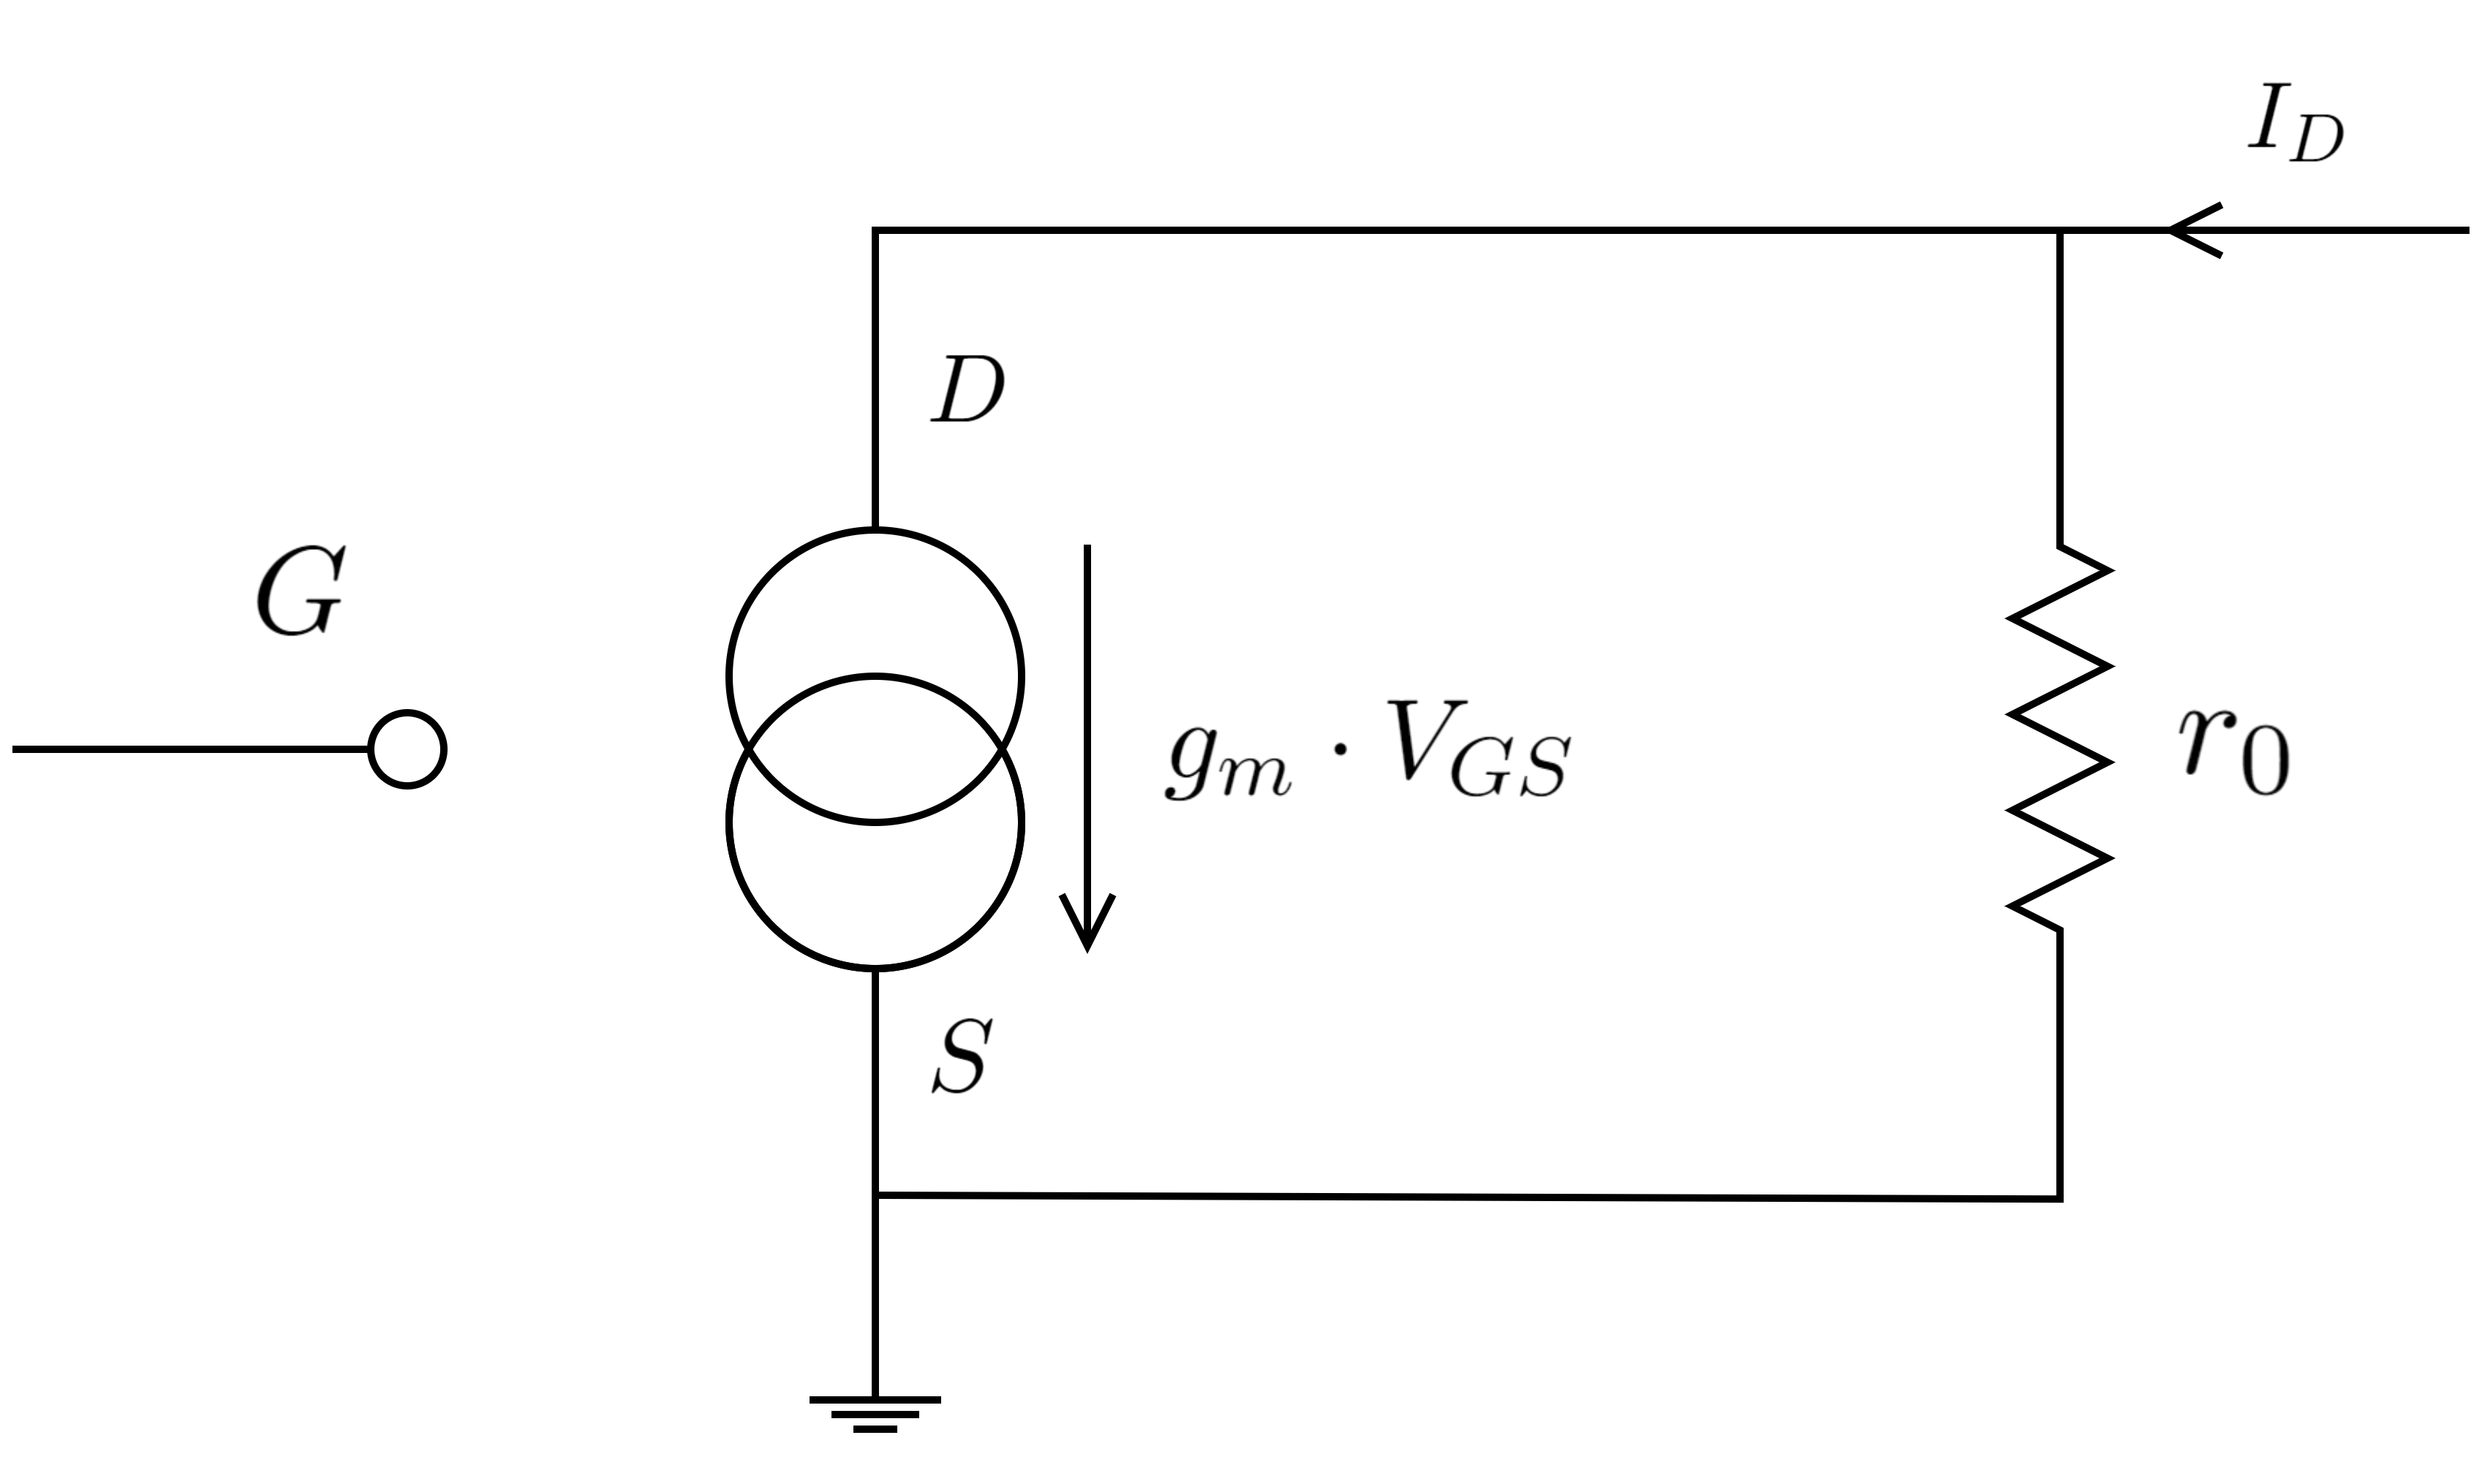
\includegraphics[width = 0.55\linewidth]{./capitolo1/MOSFET/PiccoloSegnale/PiccoloSegnale.png}
  \caption[Modello piccolo segnale]{Modello piccolo segnale}
  \label{fig:piccolo_segnale}

\end{figure}

\vspace*{0.5cm}

Per comprendere al meglio l'effettivo comportamento dei MOSFET, però, bisogna considerare che il segnale in uscita al MOSFET subisce delle interferenze dovute al rumore generato all'interno del dispositivo stesso. Esistono diverse sorgenti di rumore; qui di seguito si descrivono le principali.

\paragraph*{Rumore termico di canale}
Il canale di un dispositivo è composto da materiale resistivo e quindi è sorgente di rumore termico. Tale sorgente può essere rappresentata come un generatore di segnale con densità spettrale:

$$ S_w = 4 K_B T \frac{\alpha_w n_{sub} \gamma}{g_m} $$

\begin{itemize}
  \item la temperatura $T$. La densità spettrale è direttamente proporzionale alla temperatura assoluta,
  \item la transconduttanza di canale $g_m$, all'aumentare della quale la densità spettrale diminuisce,
  \item la lunghezza minima del canale. Infatti, al diminuire della lunghezza minima del canale, la densità spettrale può aumentare significativamente per effetto della riduzione dei portatori di carica e dell'aumento della loro temperatura.
\end{itemize}

\paragraph*{Flicker Noise}
Generalmente, a basse frequenze, prevale una componente di rumore del tipo $1/f$, la cui densità spettrale è inversamente proporzionale alla frequenza del segnale:

$$ S_{\frac{1}{f}} \left(f\right) = \frac{K_f}{C_{ox}^2 W L} \frac{1}{f^{\alpha_f}} $$

dove $K_f$ è un parametro che dipende dalla teconologia e $\alpha_f$ tiene conto della dipendenza dalla frequanza frequenza.

Le cause più probabili di questo comportamento sono: 
\begin{itemize}
  \item fluttuazione casuale del numero dei portatori di carica dovuta a fenomeni di generazione e ricombinazione, prevalente nei dispositivi a canale N,
  \item fluttuazione della mobilità dei portatori di carica a causa di fenomeni di scattering con le impurità presenti nel cristallo, prevalente nei dispositivi a canale P.
\end{itemize}

A parità di tecnologia, polarizzazione e dimensioni, il flicker noise è minore nei MOSFET a canale P, rispetto a quelli a canale N. Infine, il processo di \emph{scaling} dei dispositivi influenza la quantità di questo tipo di rumore: analizzando l'equazione della densità spettrale, si nota come la riduzione delle dimensioni del canale comportano un aumento di rumore. Al contrario, la diminuzione dello spessore del Gate porta all'aumento della sua capacità e quindi ad una riduzione del rumore. Allo stesso tempo, però, un Gate più fine è soggetto ad un maggiore degrado, quindi il fattore $K_f$ potrebbe non diminuire come aspettato. 

\paragraph*{Rumore Lorentziano}
Il rumore Lorentziano, o \emph{Random Telegraph Signal} (\emph{RTS}), è causato dall'intrappolamento e rilascio dei portatori di carica da parte di trappole presenti nella regione di svuotamento tra il canale di conduzione e l'ossido. Questo tipo di rumore è maggiormente presente nei dispositivi soggetti a grandi dosi di radiazioni e fluenze neutroniche, che producono nel reticolo cristallino dei difetti che fungono da centri di intrappolamento. La riduzione di spessore del Gate comporta un aumento del numero delle trappole, poiché soggetto a maggior degrado.

\paragraph*{Rumore associato alla corrente di Gate}
Fino ad ora si è considerata solo la corrente $I_D$ che va da dal Drain al Source (o viceversa, in base al tipo di canale). In realtà esiste anche una corrente $I_G$ che attraversa il Gate, che in generale, appunto, è trascurabile, se confrontata con  $I_D$. Infatti l'ossido presente tra la metallizzazione del Gate e il substrato fa da barriera di potenziale all'iniezione dei portatori di carica. Questa barriera può essere comunque attraversata dai portatori con temperatura (e quindi energia cinetica) maggiore. Con la riduzione dello spessore del gate, l'energia necessaria per iniettare i portatori attraverso il Gate diminuisce e quindi $I_G$ diventa meno trascurabile.

\paragraph*{Altre sorgenti di rumore}
Ci sono infine sorgenti di rumore legate alle resistenze presenti nel Gate e nel substrato e alle resistenze parassite di Drain e Source.